\documentclass[11pt,letter]{article}
\usepackage[top=0.65in,bottom=0.9in,left=0.85in,right=0.85in]{geometry}

%\def\baselinestretch{1.25}
\def\baselinestretch{1.0}

\usepackage[greek, english]{babel}
\usepackage{multicol}

\usepackage{graphicx}
\usepackage[export]{adjustbox}


% The use of the times package forces the use of the type-1 times
% roman font, but the times roman font does not look nice.
% Besides the times roman font still does not print correctly on
% the dopy printer.
%\usepackage{times}


\usepackage{fancyhdr}
\usepackage{amsmath}
\usepackage{amssymb}
\usepackage{bm}
\usepackage{bbold}
\usepackage{parskip}
\usepackage{url}
\usepackage{xfrac}
\usepackage{isomath}

\newcommand{\bv}[1]{\ensuremath{\bm{#1}}}
\newcommand{\ts}[1]{\ensuremath{\tensorsym{#1}}}
\newcommand{\vo}{\ensuremath{V_{0}}}
\newcommand{\bvo}{\ensuremath{\bv{V}_{0}}}
\newcommand{\er}{\ensuremath{E_{R}}}
\newcommand{\Lc}{\ensuremath{L_{\mathrm{c}}}}
\newcommand{\dsig}[1]{\ensuremath{ \frac{ d\,\sigma_{#1} }{d\,\Omega} }}
\newcommand{\dbl}{\ensuremath{ \uparrow\! \downarrow \, }}
\newcommand{\spup}{\ensuremath{ \uparrow }}
\newcommand{\spdn}{\ensuremath{ \downarrow}}
%\newcommand{\hhh}{\ensuremath{\left( \sfrac{1}{2}\,\sfrac{1}{2}\,\sfrac{1}{2}\right)  }}
\newcommand{\hhh}{\ensuremath{\left( \frac{1}{2}\,\frac{1}{2}\,\frac{1}{2}\right)  }}

\begin{document}

{\Large \bf Polarization phase-contrast imaging}

In this document we will introduce the technique of polarization phase-contrast
imaging (PPCI), which is used in various stages of our experiment to measure
the in-situ column density of of the dilute gas.   The general goal of atom
cloud imaging is to obtain a quantitative measure of the density distribution
of the sample by looking at the intensity, phase and polarization profiles of
light that has gone through it.    The widely used absorption imaging
technique looks at the intensity attenuation profile for a resonant, or nearly
resonant laser beam.   On the other hand, light with a larger detuning is used
for PPCI; the attenuation of the intensity can be neglected and the information
about the density of the gas can be extracted from the phase profile of the
transmitted beam.   The treatment is separated into two parts, first we
calculate the relationship between the phase shift of the transmitted light and
the column density of the cloud.   Then we examine the experimental setup which
allows one to convert the phase shift profile into an intensity profile that
can be recorded on a CCD camera.   
 
 
\section{Dielectric properties of the atom cloud}


In the following we want to find what happens with the electric field of a
laser beam as it goes through a cloud of atoms.   We treat the atom cloud as a
continous dielectric medium in which the electric field induces a polarization
$\bv{\mathcal{P}}(\bv{r}, t)$.   This polarization corresponds to the electric
dipole moment per unit volume in the cloud.  If we can calculate the electric
dipole moment induced on one atom, $\langle \bv{d}\, \rangle$, and if we know
the density of the cloud, $n(\vec{r})$, then we can simply write the induced
polarization as 
\begin{equation}
 \bv{\mathcal{P}}( \bv{r}, t ) = \langle \bv{d}\, \rangle n(\bv{r}) 
\end{equation}
The induced dipole moment on an atom is proportional to the electric
field\footnote{As long as we keep the probe laser power below the nonlinear
regime} $\bv{\mathcal{E}}$, and in the general case the proportionality is given by the electric
susceptibility tensor,  $\ts{\chi}$: 
\begin{equation} 
 \langle \bv{d}\,\rangle = \epsilon_{0}\ts{\chi} \bv{\mathcal{E}} 
\end{equation}

An ensemble of atoms (in which each atom may be in a different quantum state) is
best described using the density matrix, which is defined as \begin{equation}
  \ts{\rho} = \frac{1}{N} \sum_{i=1}^{N} | \psi_{i} \rangle \langle \psi_{i} | 
\end{equation}
where the $i^{\text{th}}$ atom in the ensemble is in state $|\psi_{i}\rangle$.
The expectation value of the electric dipole moment is then given by 
\begin{equation}
   \langle \bv{d}\, \rangle  = \text{Tr} ( \ts{\rho} \bv{d} ) 
\end{equation} 

The equation of motion for the density matrix follows from the Schrodinger
equation for the $|\psi_{i}\rangle$,  it is known as the Liouville equation,
which in the presence of relaxation from any excited states
is~\cite{auzinsh2010optically} 
\begin{equation}
  i \hbar \dot{\ts{\rho}} = 
  [\hat{H}, \ts{\rho}] - \frac{i\hbar}{2}( \ts{\Gamma} \ts{\rho} + \ts{\rho} \ts{\Gamma}) 
\end{equation}
where $\ts{\Gamma}$ is a diagonal matrix with the decay rate of each state on
the diagonal, which is included to account for spontaneous emmission.  

The Liouville equation for the density matrix will be solved by performing a
unitary transformation to a rotating frame, as is shown in Chapter 10
of~\cite{auzinsh2010optically}, but before we can proceed to define the
transformation  we must introduce the atomic states of interest in our problem,
in other words the basis in which we will represent the atomic density matrix.

\begin{figure}[h]
\centering 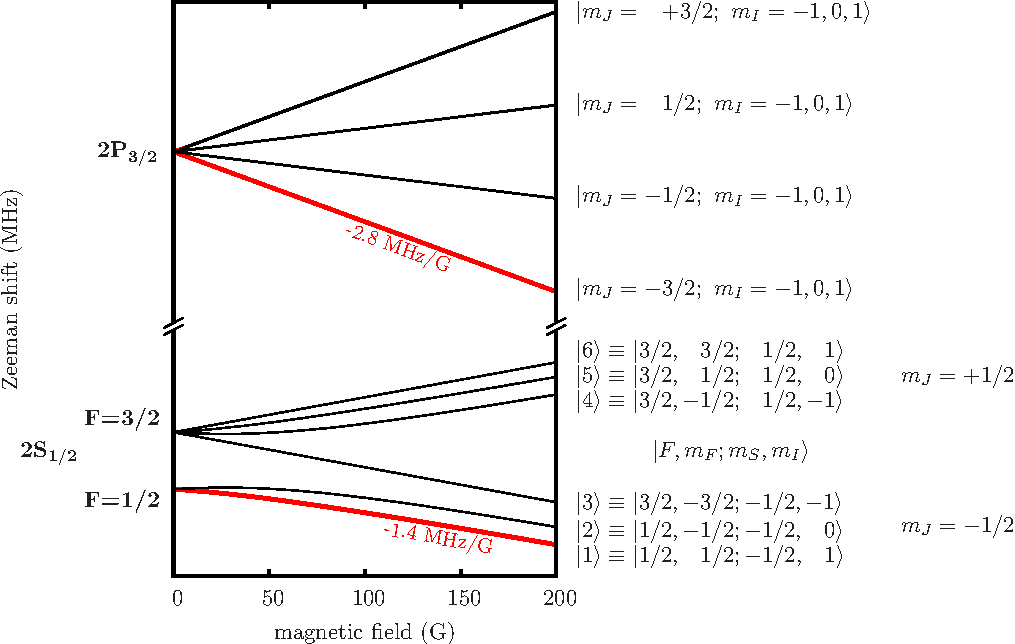
\includegraphics[width=0.85\textwidth]{01eps.pdf}
\caption[Levels relevant for imaging.]{Level diagram relevant for imaging transitions}  \label{fig:levels}
\end{figure}
Figure~\ref{fig:levels} shows the energy levels of the $2S_{1/2}$ and
$2P_{3/2}$ states of a $^{6}$Li atom in the presence of a magnetic field. In
our experiment we tipically have atoms in an incoherent spin mixure of states
$|1\rangle$ and $|2\rangle$.  The fields where we operate are typically $>300$
G, where good quantum numbers are $J,m_{J}$ and $I,m_{I}$.  In other words, the
field is high enough that the angular momentum of the valence electron is
decuopled from the angular momentum of the nucleus, and the energy of the atom
in the magnetic field is approximately $(g_{J}\mu_{B}m_{J} +
g_{I}\mu_{B}m_{I})B$.

The angular monetum projection selection rule for a one photon transition is
$\Delta m_{J} = 0, \pm 1$, which means that we can drive transitions from
states $|1\rangle$ and $|2\rangle$ (both of which have $m_{J}=-1/2$) to the
$2P_{3/2}$ excited states with $m_{J} = -3/2, -1/2, +1/2$.  We typically use
$\sigma_{-}$ polarized light, so we drive transitions to $m_{J}=-3/2$, which is
advantageous because this is a cycling transition, which means it  can only
decay back to $m_{J}=-1/2$.  In phase-contrast imaging the probe light is
detuned far enough from the atomic state that the population in the excited
state can in most cases be neglected.  The fact that the transition closer to
the probe laser is a cycling transition is thus inconseqiential.   A basic
analysis considers only the $m_{J}=-3/2$ excited states, but if the detuning is
sufficiently large, such as it is sometimes necessary for in-situ imaging of
very dense clouds,  then we must also take into account the $m_{J}=-1/2$ and
$m_{J}=+1/2$ states. 

The basis set of states thus should consist of eight states. Four of them are
state $|1\rangle$, which has a nuclear spin projection $m_{I}=+1$  plus the
three corresponding excited states $m_{J}=-3/2,-1/2,+1/2$ with $m_{I}=+1$.
The other four correspon to the $m_{I}=0$ subspace, which contains $|2\rangle$. 
Since the electric dipole does not couple the nuclear spins, we will solve the
problem in one of the $m_{I}$ substate, and the solution for the other one will
be identical.  So the basis set of states that we will consider is $\lbrace
|g\rangle, |e_{-}\rangle, |e_{0}\rangle, |e_{+}\rangle \rbrace$, where
the first is the ground state and the last three are excited states. 

The density matrix is then  
\begin{equation}
 \ts{\rho} = \left[\begin{smallmatrix}\rho_{{gg}} & \rho_{{+g}} & \rho_{{0g}} & \rho_{{-g}}\\\rho_{{g+}} & \rho_{{++}} & \rho_{{0+}} & \rho_{{-+}}\\\rho_{{g0}} & \rho_{{+0}} & \rho_{{0+}} & \rho_{{-0}}\\\rho_{{g-}} & \rho_{{+-}} & \rho_{{0-}} & \rho_{{--}}\end{smallmatrix}\right]
\end{equation}

The unperturbed Hamiltonian of the atom is 
\begin{equation}
H_{0} = \hbar \left[\begin{smallmatrix}0 & 0 & 0 & 0\\0 & \omega_{{-}} & 0 & 0\\0 & 0 & \omega_{{0}} & 0\\0 & 0 & 0 & \omega_{{+}}\end{smallmatrix}\right]
\end{equation} 

For the interaction between the atoms and the oscillating electric field of the
probe laser, we use the electric dipole Hamiltonian $H_{I} = - \bv{d} \cdot
\bv{\mathcal{E}}\cos(\omega t)$, we can expand the vectors in the spherical basis $\lbrace
\bv{e}_{\pm}, \bv{e}_{0} \rbrace$, which results in 
\begin{equation}
  H_{I} = - \left( \mathcal{E}_{x} d_{x}  
          + \mathcal{E}_{y} d_{y} + \mathcal{E}_{z} d_{z} \right) 
            \cos(\omega t )  
\end{equation} 
To evaluate the matrix for $H_{I}$ we need to find the matrix elements of
the cartesian components of $\bv{d}$.  We evaluate the the components of $\bv{d}$
in the spherical basis, $d_{q}$, where $q\in{-1,0,1}$ and then later we can
evaluate the cartesian components by projecting them onto the spherical basis
vectors.  

To evaluate the matrix elements of the $d_{q}$, the Wigner-Eckart
theorem\footnote{Sec.~5.4.1 on \cite{edmonds1996angular}} is used, in order to
make the angular momentum selection rules explicit in the 3-$j$ symbol.  This
defines the reduced matrix element $\langle e \lVert d \rVert g \rangle$,
\begin{equation}
  \langle e | d_{q} | g \rangle = 
      (-1)^{J_{e}-m_{e}} 
      \begin{pmatrix} J_{e} & 1 & J_{g} \\ -m_{Je} & q & m_{Jg} \end{pmatrix}
      \langle e \lVert d \rVert g \rangle
\end{equation}

The reduced matrix element satisfies   $\langle e \lVert d \rVert g \rangle = -
\langle g \lVert d \rVert e \rangle$, so the reader may verify that (in units of the reduced matrix element) 
\begin{equation}
    d_{-1}  = \frac{\sqrt{3}}{6}  
            \left[\begin{smallmatrix}
            0 & \sqrt{3} & 0 & 0\\
            0 & 0 & 0 & 0\\
            0 & 0 & 0 & 0\\
            -1 & 0 & 0 & 0
            \end{smallmatrix}\right] \ \ \ \
    d_{0}  =  \frac{\sqrt{6}}{6}   
              \left[\begin{smallmatrix}
              0 & 0 & 1 & 0\\
              0 & 0 & 0 & 0\\
              1 & 0 & 0 & 0\\
              0 & 0 & 0 & 0
              \end{smallmatrix}\right] \ \ \ \
    d_{1} =   \frac{\sqrt{3}}{6} 
              \left[\begin{smallmatrix}
              0 & 0 & 0 & 1\\
              -\sqrt{3} & 0 & 0 & 0\\
              0 & 0 & 0 & 0\\
              0 & 0 & 0 & 0
              \end{smallmatrix}\right]
\end{equation}
and upon using $d_{x}= \frac{1}{\sqrt{2}}( d_{-} - d_{+} )$,  $d_{y} =
\frac{i}{\sqrt{2}}( d_{-} + d_{+} )$, and $d_{z} = d_{0}$ gives
\begin{equation}
    d_{x}  = \frac{1}{2\sqrt{6}}  
            \left[\begin{smallmatrix}
            0 &  \sqrt{3} & 0 & -1\\
            \sqrt{3} & 0 & 0 & 0\\
            0 & 0 & 0 & 0\\
            -1 & 0 & 0 & 0
            \end{smallmatrix}\right] \ \ \ \ 
    d_{y} =   \frac{i}{2\sqrt{6}} 
              \left[\begin{smallmatrix}
              0 & \sqrt{3} & 0 & 1\\
              -\sqrt{3} & 0 & 0 & 0\\
              0 & 0 & 0 & 0\\
              -1 & 0 & 0 & 0
              \end{smallmatrix}\right] \ \ \ \
    d_{z}  =  \frac{1}{\sqrt{6}}   
              \left[\begin{smallmatrix}
              0 & 0 & 1 & 0\\
              0 & 0 & 0 & 0\\
              1 & 0 & 0 & 0\\
              0 & 0 & 0 & 0
              \end{smallmatrix}\right]  
\end{equation}

We know define three different Rabi frequencies as 
\begin{equation}
    \hbar\Omega_{x} = \frac{ \langle e \lVert d \rVert g \rangle \mathcal{E}_{x} }{ 2\sqrt{6}}  \ \ \ 
    \hbar\Omega_{y} = \frac{ \langle e \lVert d \rVert g \rangle \mathcal{E}_{y} }{ 2\sqrt{6}}  \ \ \ 
    \hbar\Omega_{z} = \frac{ \langle e \lVert d \rVert g \rangle \mathcal{E}_{z} }{ \sqrt{6}}  
\end{equation}
and we can write 
\begin{equation}  
  H_{I} =  \hbar \cos(\omega t) 
            \left[\begin{smallmatrix}
            0 & \ -\sqrt{3}(\Omega_{x}+i\Omega_{y})\  &\ -\Omega_{z}\ &\ (\Omega_{x}-i\Omega_{y})\ \\
            \ -\sqrt{3}(\Omega_{x}-i\Omega_{y})\ & 0 & 0 & 0\\
            \ -\Omega_{z}\ & 0 & 0 & 0\\
            \ (\Omega{x}+i\Omega_{y})\  & 0 & 0 & 0
            \end{smallmatrix}\right] 
\end{equation}

\newpage


$|\langle R_{e}\, L\,S\,J || d || R_{g}\,
L\,S\,J
\rangle|^{2}$, 
\begin{align} |\langle e | d_{q} | g \rangle|^{2} & =
\begin{pmatrix} J_{e} & 1 & J_{g} \\ -m_{Je} & q & m_{Jg} \end{pmatrix}^{2}
|\langle R_{e}\, L\,S\,J || d || R_{g}\, L\,S\,J \rangle|^{2} 
\end{align} 
The
dipole moment operator only acts on the electronic angular momentum, $L$, and
our quantum state is expressed in the $LS$ coupled scheme, where $L$ and $S$
are coupled to form $J=L+S$.  One can use the formula for the expectation of a
single part operator on a coupled scheme\footnote{Sec.~7.1.7 on
\cite{edmonds1996angular}}, in this case the dipole moment operating on the
$LS$ coupled state. One obtains \begin{align} |\langle e | d_{q} | g
\rangle|^{2} & = \begin{pmatrix} J_{e} & 1 & J_{g} \\ -m_{Je} & q & m_{Jg}
\end{pmatrix}^{2} (2J_{e}+1)(2J_{g}+1)  \begin{Bmatrix}L_{g} & J_{g} & S \\
J_{e} & L_{e} & 1 \end{Bmatrix}^{2}|\langle R_{e}\, L || d || R_{g}\, L
\rangle|^{2} \end{align} The fully reduced matrix element can be related to the
lifetime, $\tau$, or the natural linewidth, $\Gamma$, of the excited
state~\cite{Olivares:98}, \[ |\langle R_{e}\, L || d || R_{g}\, L \rangle|^{2}
= \frac{1}{\tau} \frac{ 9\epsilon_{0} \hbar \lambda^{3}}{8 \pi^{2}} =
\Gamma\frac{ 9\epsilon_{0} \hbar \lambda^{3}}{8 \pi^{2}} \] resulting finally
in \begin{align} |\langle e | d_{q} | g \rangle|^{2} & = \begin{pmatrix} J_{e}
& 1 & J_{g} \\ -m_{Je} & q & m_{Jg} \end{pmatrix}^{2} (2J_{e}+1)(2J_{g}+1)
\begin{Bmatrix}L_{g} & J_{g} & S \\ J_{e} & L_{e} & 1
\end{Bmatrix}^{2}\Gamma\frac{ 9\epsilon_{0} \hbar \lambda^{3}}{8 \pi^{2}}
\end{align} At this point we plug in some of the values for our case,
$L_{g}=0$, $J_{g} = 1/2$, $m_{Jg}=-1/2$, $L_{e}=1$, and $J_{e}=3/2$.  The $6j$
symbol can be evaluated in Mathematica.  This results in,


\newpage
 

 We perform a transformation to the rotating
frame using the unitary matrix $U$, 

where the  electron's wave function is:
and the equation of motion for the  $c$ coefficients is derived from the
Schrodinger equation: 
\begin{equation}
 i \hbar \dot{c}_{k}(t) = 
 \sum_{m} c_{m}(t)e^{-i(E_{m}-E_{k})t/\hbar} 
 \langle k | \hat{H}_{\mathrm{int}}(t) | m \rangle 
\end{equation}


The interaction between the atom and the electric field is given by
the optical Bloch equations, an
$\hat{H}_{\mathrm{int}}(t)  = -\bv{d}\cdot\bv{E} \cos( \omega t )$.  It is
useful to define the density matrix $\rho_{mn} = c_{n}^{*}c_{m}$, which has the
following equation of motion 
\begin{equation}
\dot{\rho}_{mn} = 
    \frac{1}{i\hbar} \sum_{l}  \left( 
    \rho_{ln} e^{-i ( E_{l}-E_{m})t/\hbar } 
    \langle m  | \hat{H_{\text{int}}} | l \rangle 
  -  \rho_{ml} e^{i(E_{l}-E_{n}) t/ \hbar } 
    \langle  l | \hat{H_{\text{int}}} | n \rangle 
    \right) 
\end{equation} 



\section{Experimental setup for PPCI} 



\bibliographystyle{osa}
\bibliography{phasecon}

\end{document}




